\documentclass[10pt,conference]{IEEEtran}
\usepackage{amsmath,amssymb,amsfonts}
\usepackage{booktabs}
\usepackage{multirow}
\usepackage{graphicx}
\usepackage{cite}
\usepackage{xcolor}
\usepackage{url}
\usepackage{enumitem}
\usepackage{microtype}

\newcommand{\N}{\mathrm{N}}
\newcommand{\R}{\mathrm{R}}
\newcommand{\Sstall}{\mathrm{S}}
\newcommand{\risk}{\mathcal{R}}
\newcommand{\sysname}{\textsc{ProgressRisk}}

\title{Sensing PBFT Progress Without Identifying Validators:\\
Risk-Aware Random Reconfiguration for Sharded BFT Systems}

\author{\IEEEauthorblockN{Anonymous Authors}
\IEEEauthorblockA{Working manuscript --- author names omitted}}

\begin{document}
\maketitle

\begin{abstract}
Random committee assignment is a foundational defense in sharded blockchains: when adversarial identities are unknown, randomization probabilistically disperses Byzantine validators. Yet a safe global adversarial fraction does not preclude a dangerous local concentration in one committee. Existing sharding systems therefore either rely on large committees, tolerate corrupted shards after they occur, or recover from confirmed failures. This paper asks a different question: can a sharded BFT system sense which committee is operationally risky \emph{without} identifying individual Byzantine validators, and use that evidence to make a small, budgeted reconfiguration before a local threshold failure persists?

We introduce \sysname, a PBFT-progress observation and control framework. Each logical batch is classified exactly once as normal completion, recovery-assisted completion, or operational stall. These mutually exclusive outcomes avoid treating timeout, \textsc{view-change}, and \textsc{new-view} messages as independent evidence even though they form one recovery chain. Under a declared persistent-withholding threat model and visible network/workload context, \sysname computes an exact constrained Bayesian posterior over shard-level active blocking loads and a discrete attack-intensity regime. A finite controller then selects at most one random $k$-for-$k$ validator exchange between a posterior-hot shard and a lower-risk partner.

In a controlled PBFT-style event simulation with 198 validators and 9 committees, we first use a paired development sweep to select a small exchange budget, then evaluate on 24 previously unseen random seeds. The proposed controller reduces the mean fraction of epochs containing an over-threshold shard from $0.792$ to $0.203$, while moving $2.56$ validators per epoch on average. The paper explicitly limits this result to the declared model and simulation; membership-handoff measurements on a BFT implementation remain future validation.
\end{abstract}

\begin{IEEEkeywords}
Blockchain sharding, PBFT, Byzantine fault tolerance, Bayesian inference, reconfiguration, random committee exchange.
\end{IEEEkeywords}

\section{Introduction}

Blockchain sharding improves scalability by partitioning validators and workloads into committees that execute in parallel. Randomized committee formation is a natural security baseline when validator identities are not known: systems such as OmniLedger and RapidChain use randomness to form statistically representative committees and to reduce the probability that any one committee is adversarially dominated \cite{omniledger,rapidchain}. However, this guarantee is probabilistic and local. Even when the global Byzantine fraction satisfies the usual bound, sampling variation can place too many adversarial validators in one shard. Han \emph{et al.} formalize this concern as a shard-allocation problem and identify the single-shard takeover attack \cite{han2022allocation}.

Recent work has made clear that corrupted shards are not merely a theoretical nuisance. CoChain and SpiralShard permit some small shards to be corrupted but constrain their impact through cross-shard mechanisms, while Levee detects, isolates, and recovers faulty shards \cite{cochain,spiralshard,levee}. These designs are valuable, but they primarily address how a system should survive or constrain a shard after it becomes faulty. They do not directly answer how a system can use its ordinary BFT execution traces to prioritize a modest, preemptive reshuffling when validator identities remain hidden.

The difficulty is observational. A timeout can arise from a malicious primary, a benign network delay, workload stress, or a crash. Moreover, timeout, \textsc{view-change}, and \textsc{new-view} are usually consecutive elements of one liveness-recovery process, not independent pieces of evidence. Directly multiplying their counts in a Bayesian model both double-counts an event chain and leaves the log-to-Byzantine likelihood underspecified.

We address this issue by moving the observation boundary from individual log messages to a logical batch's final PBFT progress outcome. PBFT executes a request only after it reaches the commit condition; a client accepts the result after receiving matching replies. If progress does not occur, timeout drives view recovery through \textsc{view-change} and \textsc{new-view} \cite{castro1999pbft}. Accordingly, a batch is observed as: (i) \emph{normal} when it completes in the initial view, (ii) \emph{recovered} when it completes only after an installed new view, or (iii) \emph{stalled} when it remains incomplete at the control deadline. RBFT further motivates using progress degradation rather than only overt safety violations: a malicious primary can harm BFT performance without violating safety rules \cite{aublin2013rbft}.

\paragraph{Contributions.} This working draft makes four contributions.
\begin{enumerate}[leftmargin=13pt,itemsep=1pt]
\item We define a protocol-grounded, mutually exclusive observation alphabet $\{\N,\R,\Sstall\}$ for logical PBFT batches, separating final progress outcomes from the internal recovery events that produce them.
\item Under an explicit persistent-withholding threat model, visible context, and a configuration-time active-load budget, we derive an exact constrained Bayesian posterior over shard-level active quorum-blocking loads. The exact dynamic program avoids static-particle resampling collapse in the threshold tail.
\item We design a deployable finite action controller. It selects an action $a=(h,c,k)$: randomly exchange $k$ validators between a posterior-hot shard $h$ and a lower-risk shard $c$, or take no action. The controller never identifies individual validators.
\item We implement a controlled PBFT-style event simulator and evaluate the signal, its context negative control, calibration, and policy impact. The current results are restricted to controlled simulation and are reported with their limitations.
\end{enumerate}

\section{Background and Motivation}

\subsection{PBFT progress and view recovery}

In PBFT, a client request follows the normal sequence
\begin{equation}
\begin{aligned}
\textsc{Request} &\rightarrow \textsc{Pre-Prepare} \rightarrow \textsc{Prepare} \\
&\rightarrow \textsc{Commit} \rightarrow \textsc{Execute} \rightarrow \textsc{Reply}.
\end{aligned}
\end{equation}
For a committee of $n=3f+1$ replicas, a replica commits locally after it is prepared and obtains $2f+1$ matching commit messages; the client accepts after $f+1$ matching replies \cite{castro1999pbft}. A replica that waits too long for execution starts the view-change procedure, which installs a new primary and continues progress.

PBFT therefore provides a precise semantics for system progress but not a free Byzantine-identification oracle. A stalled request is evidence that progress failed within a window; it does not by itself establish why. \sysname uses the PBFT lifecycle to define what is observed, and places assumptions about attacker behavior and benign context explicitly in the likelihood.

\subsection{Why local risk matters in sharding}

Random committee assignment is widely used because it disperses adversaries in expectation \cite{omniledger,rapidchain}. Yet local tail events matter: compromising one shard can threaten a sharded ledger even when the network-wide adversarial fraction is acceptable \cite{han2022allocation}. Existing designs handle this tension in complementary ways. CoChain employs cross-shard ``consensus on consensus'' to supervise corrupted shards \cite{cochain}; SpiralShard allows corrupted shards but requires linked cross-shard endorsement before finalization \cite{spiralshard}. \sysname is not a replacement for such global-resilience mechanisms. Its narrower goal is to reduce the persistence of a locally risky committee using only a small membership budget.

\section{Problem and Threat Model}

\subsection{System model}

The network has $K$ equal-size shard committees. Each committee has $n=3f+1$ validators and processes logical transaction batches during epochs. Reconfiguration is permitted only at an epoch boundary. A reconfiguration exchanges the same number of validators in both directions, so committee size and the PBFT threshold remain unchanged.

The controller observes, for each shard, its batch outcomes and a context vector $\xi_{s,t}$ containing visible covariates such as a network-stress label, timeout configuration, workload class, and batch size. The controller does \emph{not} observe validator identities, Byzantine identities, or the simulator's true shard counts.

\subsection{Persistent active-withholding adversary}

The principal threat model contains a fixed set of Byzantine validators. During the evaluation window, each such validator persistently participates in a declared withholding strategy: when selected as primary it may withhold \textsc{pre-prepare}; as a backup it may withhold timely prepare/commit participation. Let
\begin{equation}
A_s \in \{0,\ldots,n\}
\end{equation}
be the number of persistent active blockers in shard $s$. $A_s$ is \emph{not} the total number of latent Byzantine validators in arbitrary deployments. A dormant or intermittently activated Byzantine validator lies outside the current inference target.

We assume a configuration-time active-load budget $L$, such that
\begin{equation}
\sum_{s=1}^{K} A_s=L.
\end{equation}
$L$ is a threat-model parameter, not an identity oracle. The main evaluation examines robustness to a small misspecification of this budget; a general intermittent-adversary model would require an explicit hidden-state transition and is outside this draft.

\subsection{Objective}

The controller aims to reduce the frequency of epochs containing at least one shard with $A_s>f$, subject to a small migration budget. This is a local liveness-risk objective, not a claim to eliminate all Byzantine behavior or to guarantee that every random exchange improves every possible configuration.

\section{PBFT Progress Observation Model}

\subsection{Batch-level observation}

Each real pending logical batch $b$ is tracked across views using a stable batch identifier. Figure~\ref{fig:observation} defines the three outcomes:
\begin{align}
O_b=\N &\iff \text{$b$ completes in its initial view},\\
O_b=\R &\iff \text{$b$ completes after $\geq 1$ installed new view},\\
O_b=\Sstall &\iff \text{$b$ remains incomplete by deadline }D_b.
\end{align}
The deadline is a control-window definition, for example an epoch boundary or bounded recovery budget; $\Sstall$ does not assert permanent loss of liveness.

\begin{figure}[t]
\centering
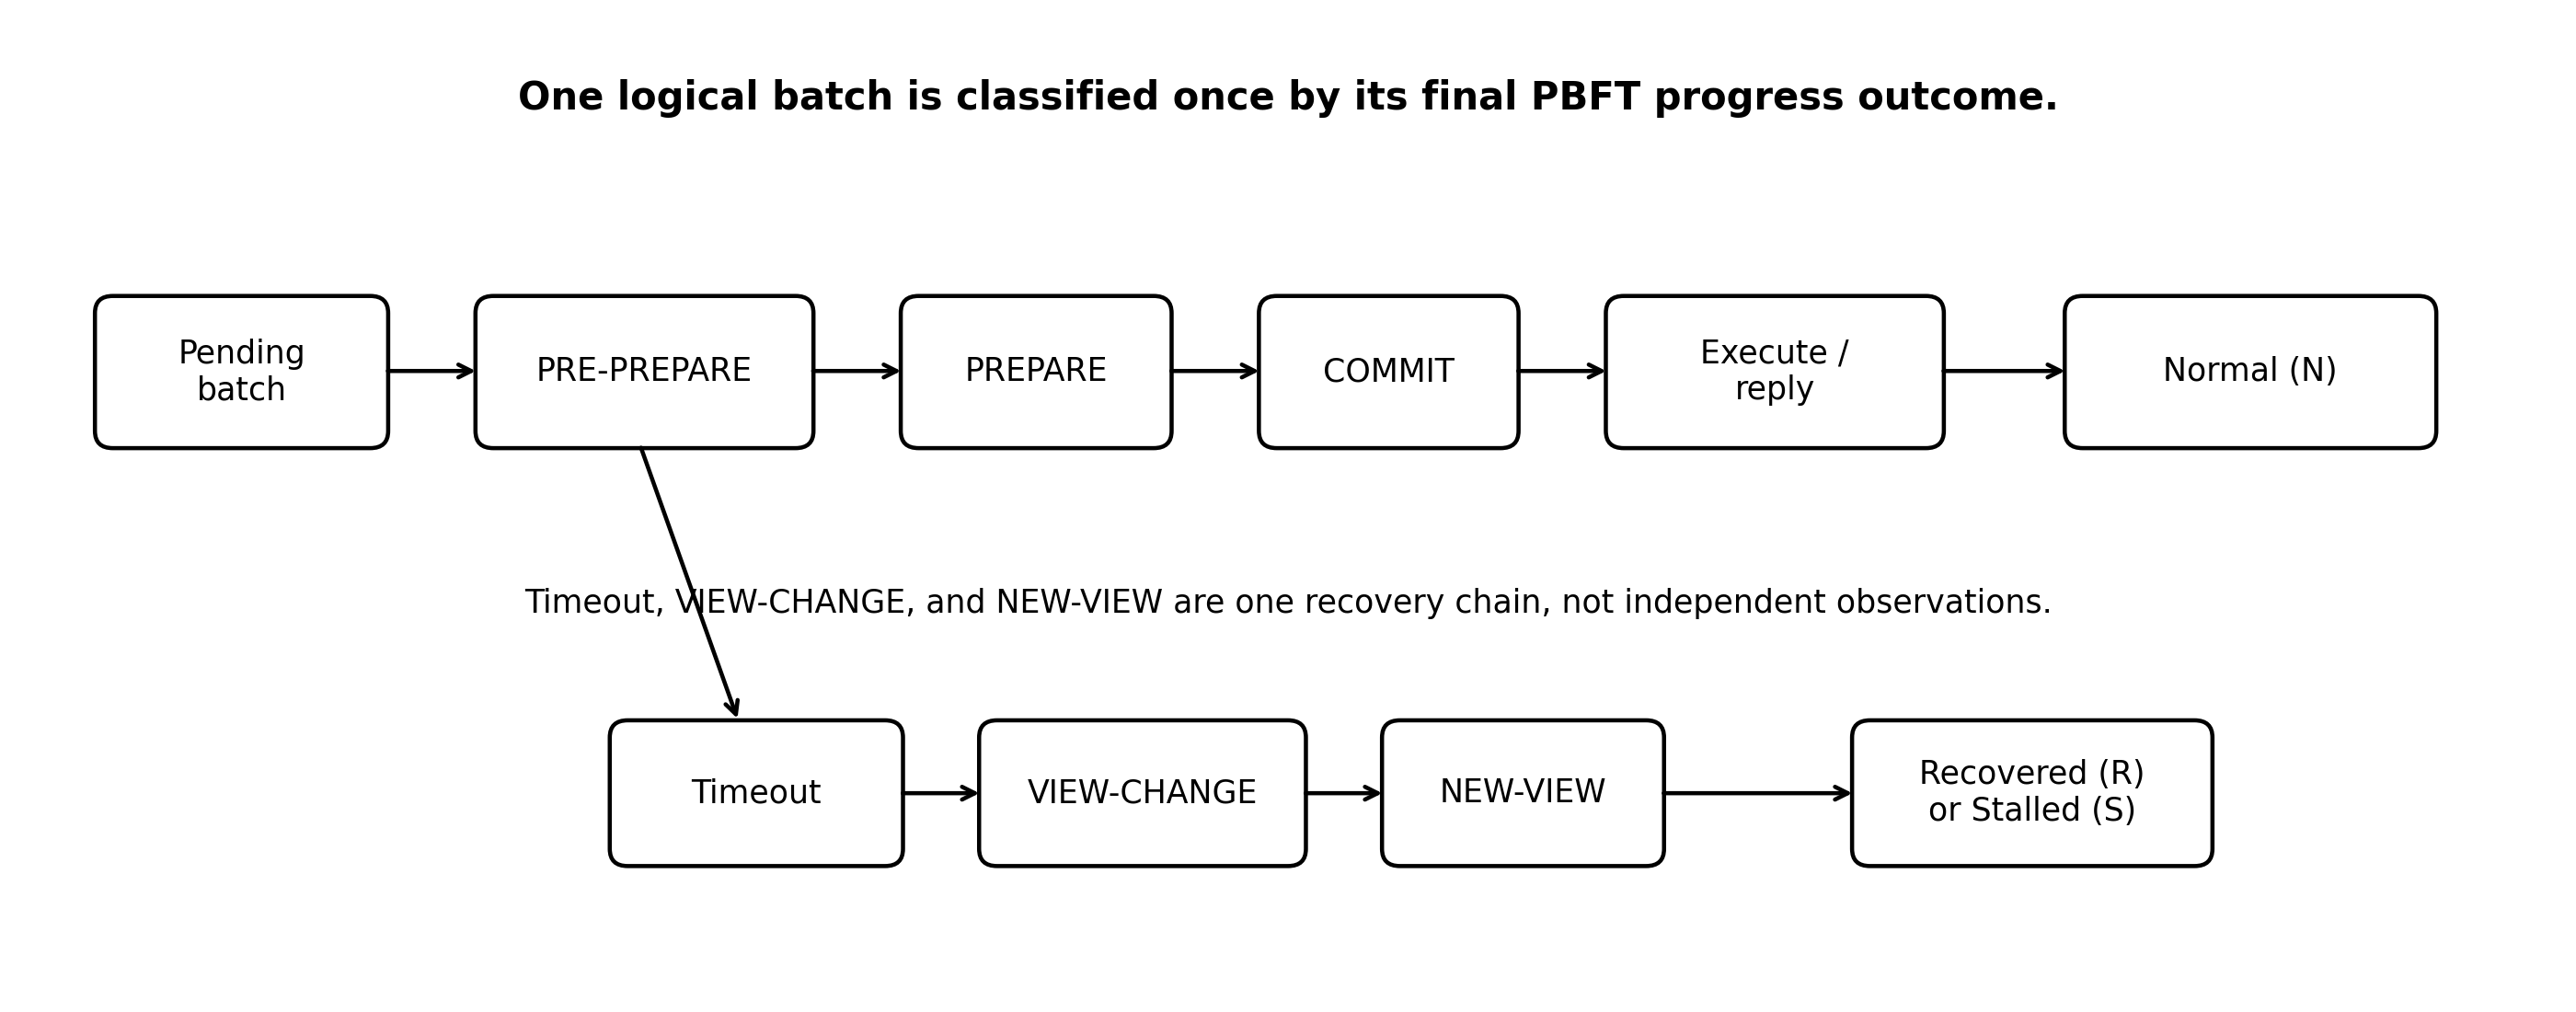
\includegraphics[width=\columnwidth]{figures/observation_pipeline.png}
\caption{\sysname observes each logical batch once, at its final progress outcome. Internal timeout and view-recovery messages are diagnostic traces rather than independent Bayesian evidence.}
\label{fig:observation}
\end{figure}

For shard $s$ in epoch $t$, $B_{s,t}$ pending batches produce the count vector
\begin{equation}
Y_{s,t}=(N^{\N}_{s,t},N^{\R}_{s,t},N^{\Sstall}_{s,t}),
\quad \sum_o N^o_{s,t}=B_{s,t}.
\end{equation}

\subsection{Context-calibrated likelihood}

Given active load $a$, context $\xi$, and attack-intensity regime $\gamma$, define
\begin{equation}
\phi_o(a,\xi,\gamma)=\Pr(O_b=o\mid A_s=a,\xi,\gamma),
\quad o\in\{\N,\R,\Sstall\}.
\end{equation}
We estimate $\phi$ offline by repeatedly executing the declared PBFT-style view chain. A view can fail because an active primary withholds, active backups withhold timely votes, or an honest replica misses a deadline according to visible context. Failed views trigger timeout and recovery; a batch stalls only when its recovery budget is exhausted.

Conditioned on a homogeneous epoch context,
\begin{equation}
Y_{s,t}\mid A_s=a,\xi_{s,t},\gamma
\sim \mathrm{Multinomial}(B_{s,t},\boldsymbol{\phi}(a,\xi_{s,t},\gamma)).
\end{equation}
This is not a universal protocol theorem. It is a calibrated generative model whose validity is evaluated against the same declared attack and context conditions.

\subsection{Exact constrained posterior}

Let $\Gamma$ be a small grid of persistent attack-intensity regimes. Conditional on the global budget $L$, the random-assignment prior over the vector $\mathbf{A}=(A_1,\ldots,A_K)$ is multivariate hypergeometric. The posterior is
\begin{equation}
\begin{aligned}
\Pr(\mathbf{A},\gamma\mid \mathbf{Y},\boldsymbol{\xi},L)
&\propto \mathbf{1}\!\left\{\sum_s A_s=L\right\}\Pr(\gamma) \\
&\quad\times \prod_{s=1}^{K}\binom{n}{A_s}\Pr(Y_s\mid A_s,\xi_s,\gamma).
\end{aligned}
\label{eq:posterior}
\end{equation}

Rather than a static particle filter, \sysname computes the posterior marginals in \eqref{eq:posterior} exactly with a forward-backward convolution over the global budget $L$. The controller's shard risk is
\begin{equation}
\risk_{s,t}=\Pr(A_s>f\mid\mathbf{Y}_t,\boldsymbol{\xi}_t,L).
\label{eq:risk}
\end{equation}
This epoch-reset posterior deliberately avoids carrying a stale latent count distribution across a membership exchange. The next epoch recomputes \eqref{eq:posterior} from fresh observed outcomes and the declared budget.

\section{Budgeted Risk-Aware Random Exchange}

\subsection{Action space}

The controller does not search for a specific ``bad'' validator. Its action is
\begin{equation}
a=(h,c,k),
\end{equation}
where $h$ is the shard with maximal posterior risk, $c$ is one of the lower-risk partner shards, and $k$ validators are sampled uniformly without replacement from both committees and exchanged.

For a posterior draw $(A_h,A_c)$, the numbers of active blockers moved out of the two committees follow hypergeometric distributions. The controller propagates posterior samples through this random exchange and estimates the maximum post-exchange risk. It selects
\begin{equation}
a^*=\arg\max_{a\in\mathcal{A}}
\left[-\widehat{\max_s\risk_s^+(a)}-\lambda\frac{2k}{N}\right],
\label{eq:utility}
\end{equation}
provided the predicted improvement exceeds a minimum threshold. Otherwise, it takes no action.

\subsection{Complexity}

For $G$ attack regimes and global budget $L$, exact inference uses truncated convolutions over $K$ committees. Its practical cost is small for the committee sizes considered here. Candidate evaluation samples a finite posterior set and considers at most $r\cdot k_{\max}$ actions, where $r$ is the number of low-risk partners. In our 198-validator simulation, the controller averaged about $56$ ms per epoch; this is a simulator measurement, not a production handoff latency.

\section{Evaluation}

\subsection{Questions and setup}

We ask:
\begin{itemize}[leftmargin=13pt,itemsep=1pt]
\item \textbf{Q1:} Do PBFT progress outcomes distinguish high active blocking load from benign network degradation when context is supplied?
\item \textbf{Q2:} Is the posterior calibrated under the declared simulation model?
\item \textbf{Q3:} Does risk-aware random exchange reduce true local threshold failures relative to random and periodic baselines?
\end{itemize}

Our controlled simulator uses $N=198$ validators in $K=9$ committees of $n=22=3\cdot7+1$ validators. The global persistent active fraction is $0.24$ ($L=48$), 72 logical batches are processed per shard per epoch, and each run lasts 24 epochs. The likelihood averages three withholding regimes: $(0.55,0.45)$, $(0.70,0.60)$, and $(0.90,0.75)$ for primary and backup withholding probabilities.

\textbf{Parameter-selection protocol.} A paired 12-seed development sweep compares $k_{\max}\in\{1,3,6,9\}$. We lock $k_{\max}=3$ before the main evaluation because it is the migration-efficiency knee: it attains a 0.184 failure-epoch fraction with 2.49 moved validators per epoch, while $k_{\max}=6$ and 9 move 5.47 and 8.79 validators for only small additional gains. All main-policy results below use 24 previously unseen seeds and the locked $k_{\max}=3$ setting.

Baselines are: (i) no reconfiguration, (ii) periodic global reshuffling every four epochs, (iii) random local exchange, and (iv) a risk-triggered policy that selects the partner shard uniformly at random after using the same trigger. The proposed policy alone selects both the partner and exchange size using \eqref{eq:utility}.

\subsection{Held-out policy comparison}

Table~\ref{tab:policy} and Figure~\ref{fig:policy} report the held-out result. The proposed controller reduces the failure-epoch fraction from $0.792$ with no reconfiguration to $0.203$. A paired bootstrap over the 24 common, previously unseen seeds gives an absolute reduction of $0.589$ with 95\% interval $[0.432,0.731]$. Relative to the risk-triggered random-partner baseline, the paired reduction is $0.203$ ($[0.123,0.285]$). It moves 2.56 validators per epoch on average, substantially less than periodic global reshuffling.

\begin{table}[t]
\caption{Held-out controlled-simulation policy comparison (24 unseen seeds, locked $k_{\max}=3$). ``Failure epochs'' is the fraction of epochs containing at least one true $A_s>f$ shard.}
\label{tab:policy}
\centering
\scriptsize
\resizebox{\columnwidth}{!}{%
\begin{tabular}{lccc}
\toprule
Policy & Failure epochs & Moved/epoch & Controller ms \\
\midrule
No reconfiguration & 0.792 & 0.00 & 6.37 \\
Periodic global reshuffle & 0.806 & 49.50 & 0.87 \\
Random local exchange & 0.769 & 3.95 & 0.89 \\
Risk-triggered random partner & 0.406 & 3.58 & 51.58 \\
\textbf{Risk-aware exchange} & \textbf{0.203} & \textbf{2.56} & 51.27 \\
\bottomrule
\end{tabular}%
}
\end{table}

\begin{figure}[t]
\centering
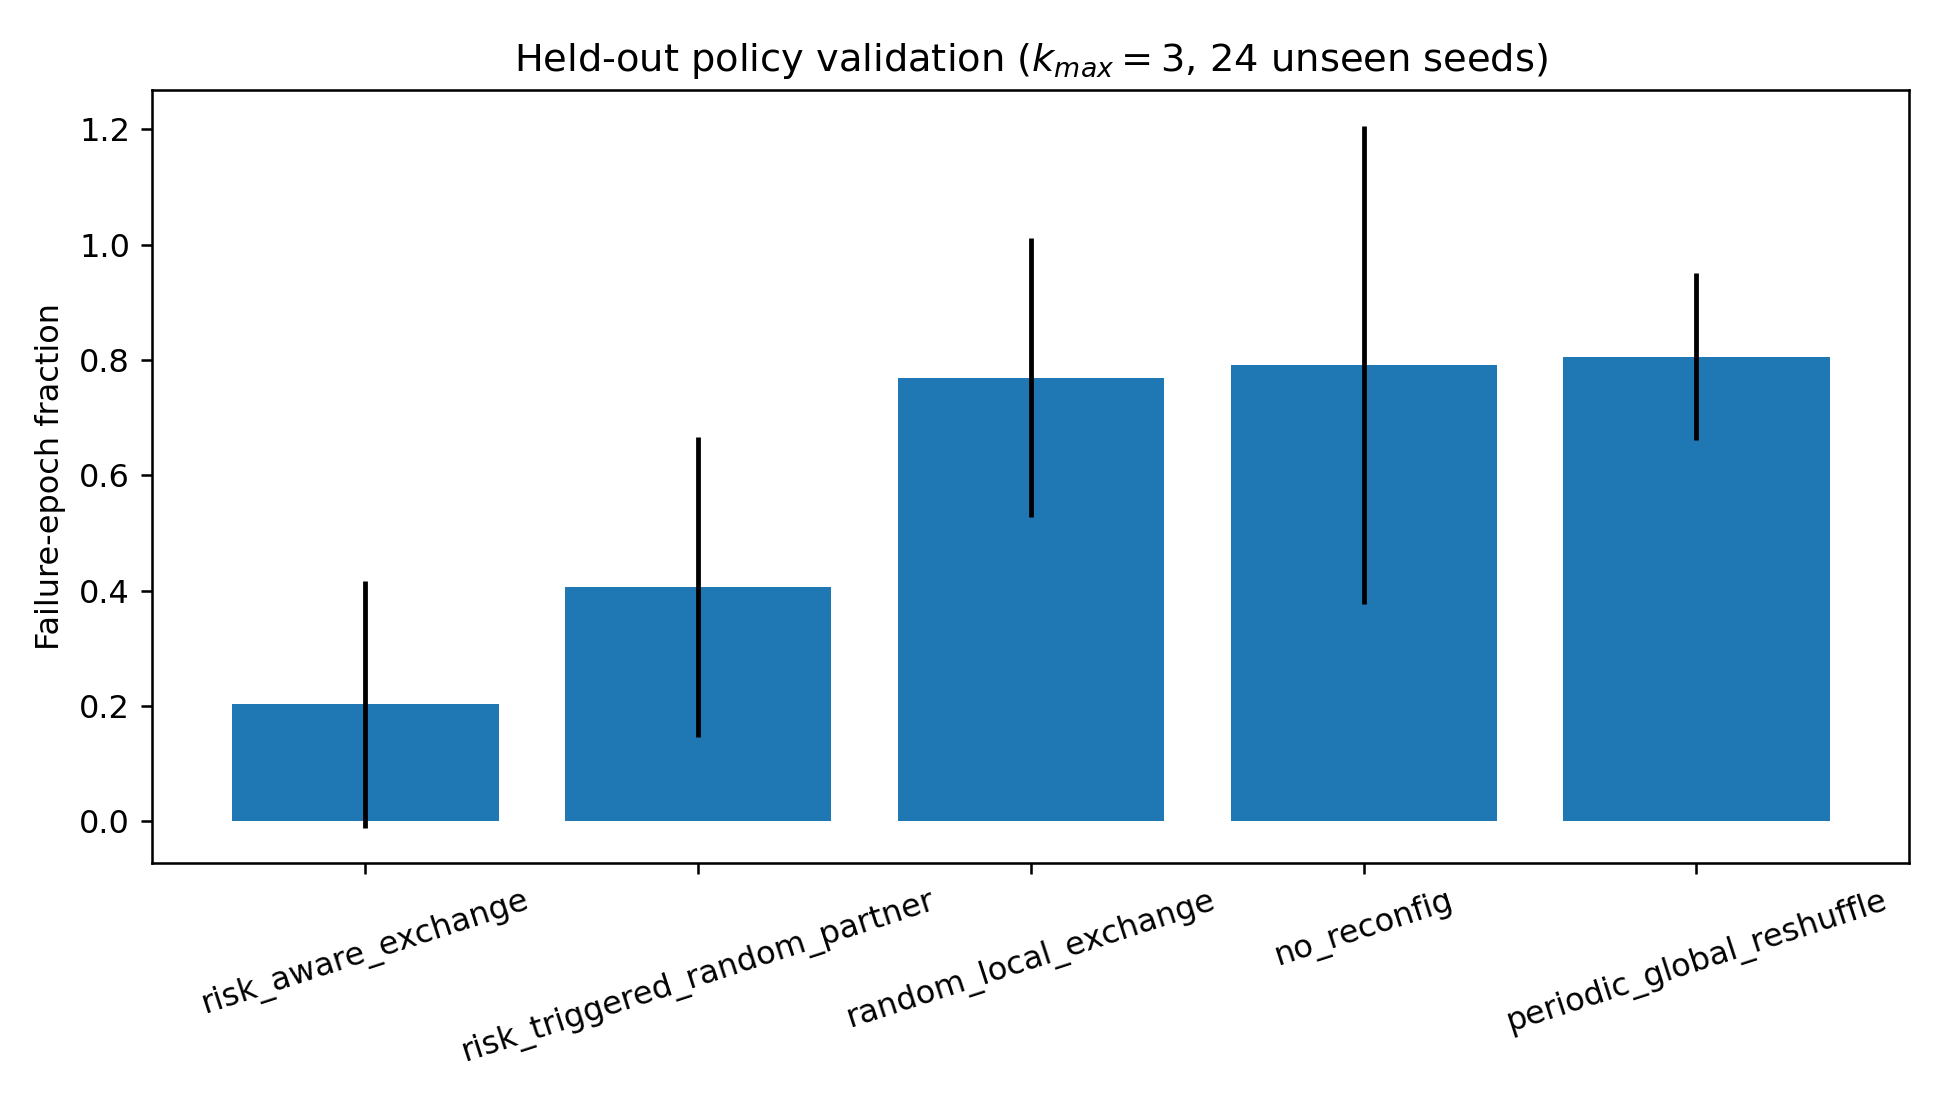
\includegraphics[width=\columnwidth]{figures/heldout_policy.png}
\caption{Held-out policy validation. Error bars show standard deviation across 24 unseen seeds.}
\label{fig:policy}
\end{figure}

The result also separates two effects. Random exchange alone has no reliable benefit in this setting; it can move active blockers in either direction. Risk triggering helps, but choosing the partner shard randomly remains weaker than posterior-guided partner selection. Thus the outcome is not simply an artifact of moving validators more often.

\subsection{Observation controls and calibration}

Figure~\ref{fig:context} is a negative control. Benign localized network degradation produces the same visible symptoms that might otherwise resemble withholding. When its context is supplied to the likelihood, the mean posterior threshold risk is effectively zero in this controlled test. If the context label is intentionally omitted, the same trace is classified as high risk. Under active withholding with normal context, the mean posterior risk is $0.694$ across 80 trials. This result does not prove deployment robustness, but it demonstrates why the context term in the likelihood is necessary rather than cosmetic.

\begin{figure}[t]
\centering
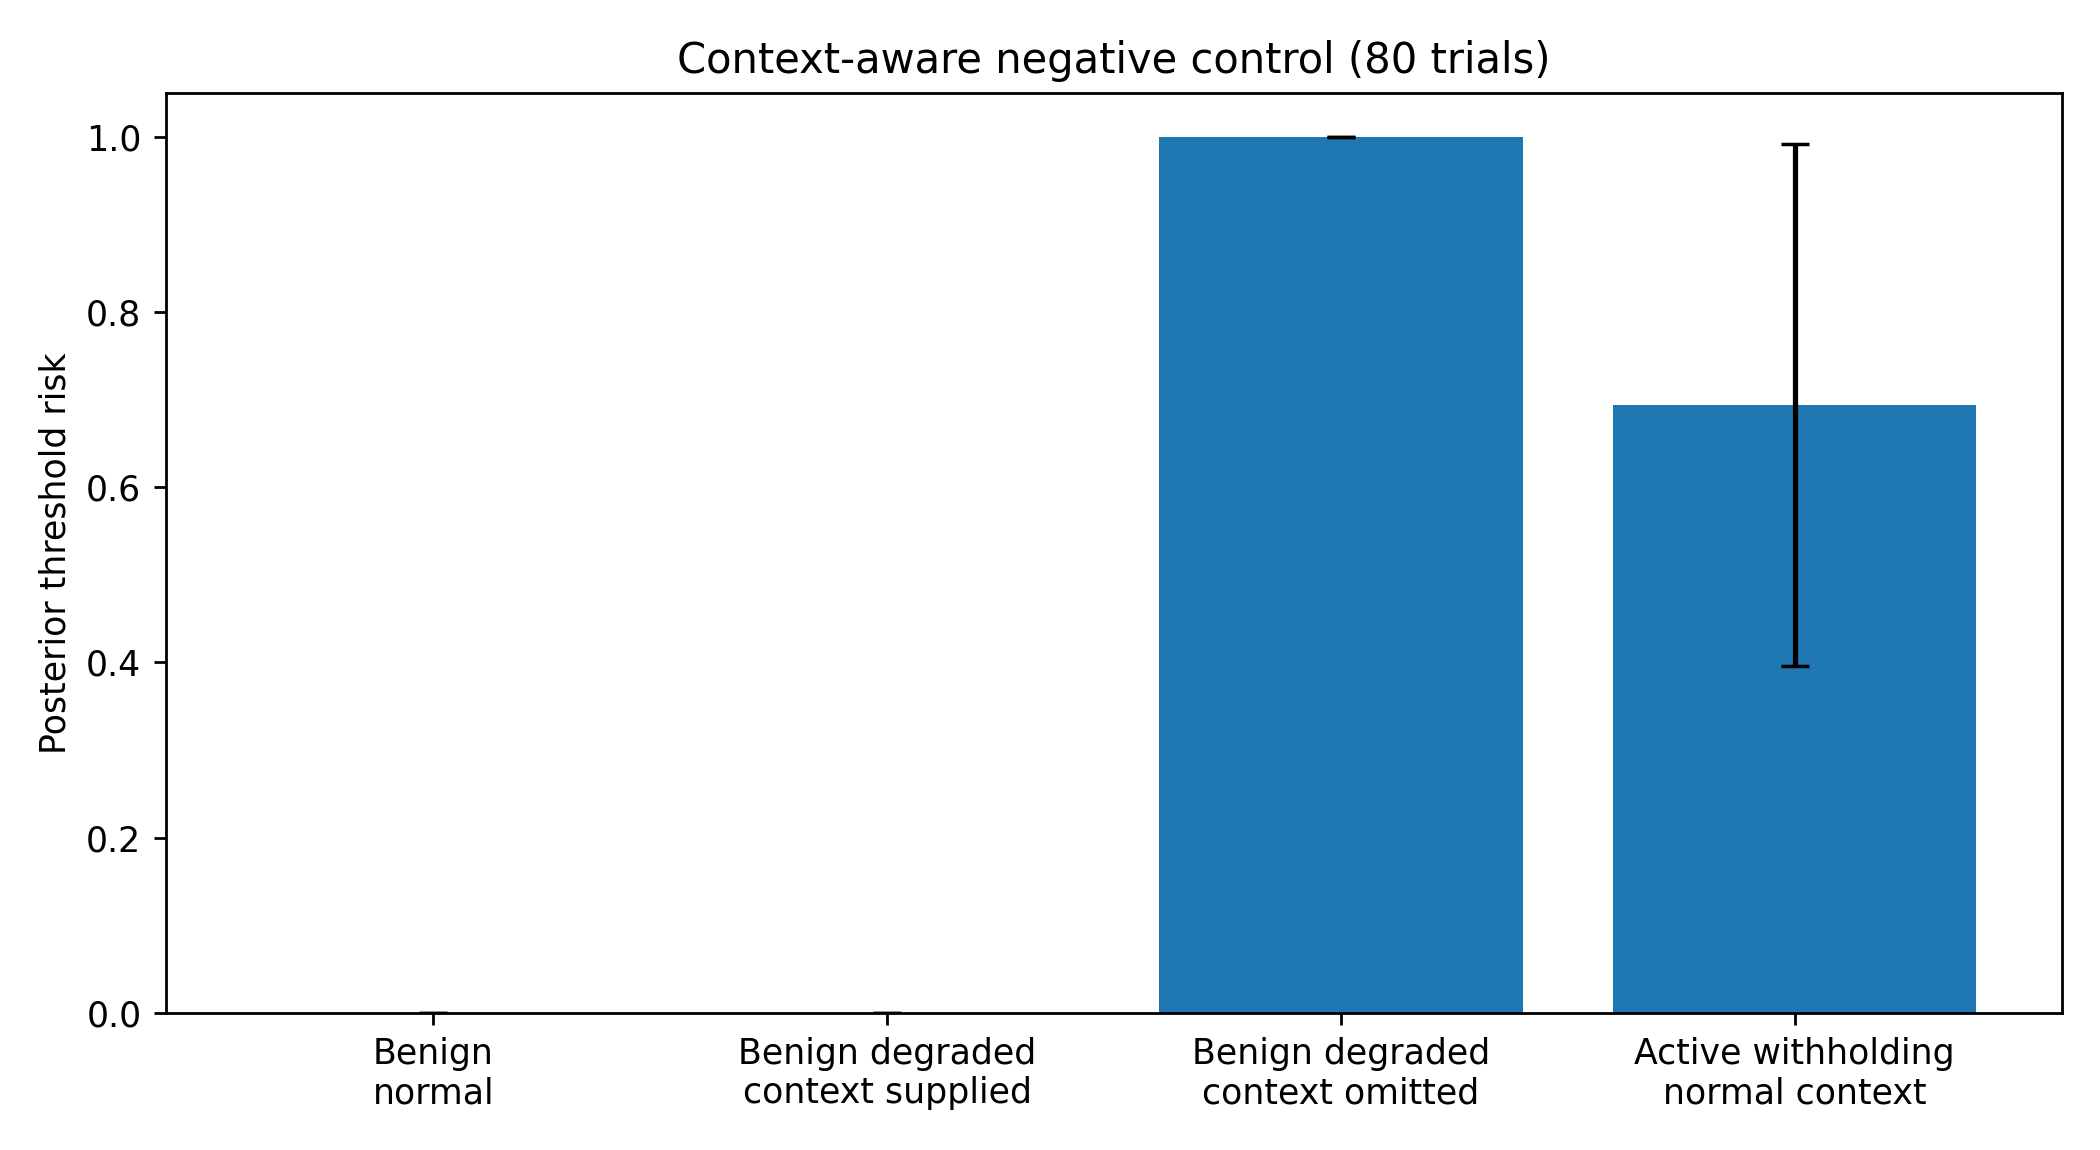
\includegraphics[width=\columnwidth]{figures/context_negative_control.png}
\caption{Context negative control. The same benign degradation trace is not attributed to active blocking when visible context is provided; omitting context causes systematic false alarms.}
\label{fig:context}
\end{figure}

On 12 no-intervention seeds under the matched simulation model, the expected calibration error is 0.003. Figure~\ref{fig:calibration} shows predicted versus observed threshold frequency. This is an internal calibration check, not external validation: likelihood calibration and test traces share the declared PBFT-style simulator.

\begin{figure}[t]
\centering
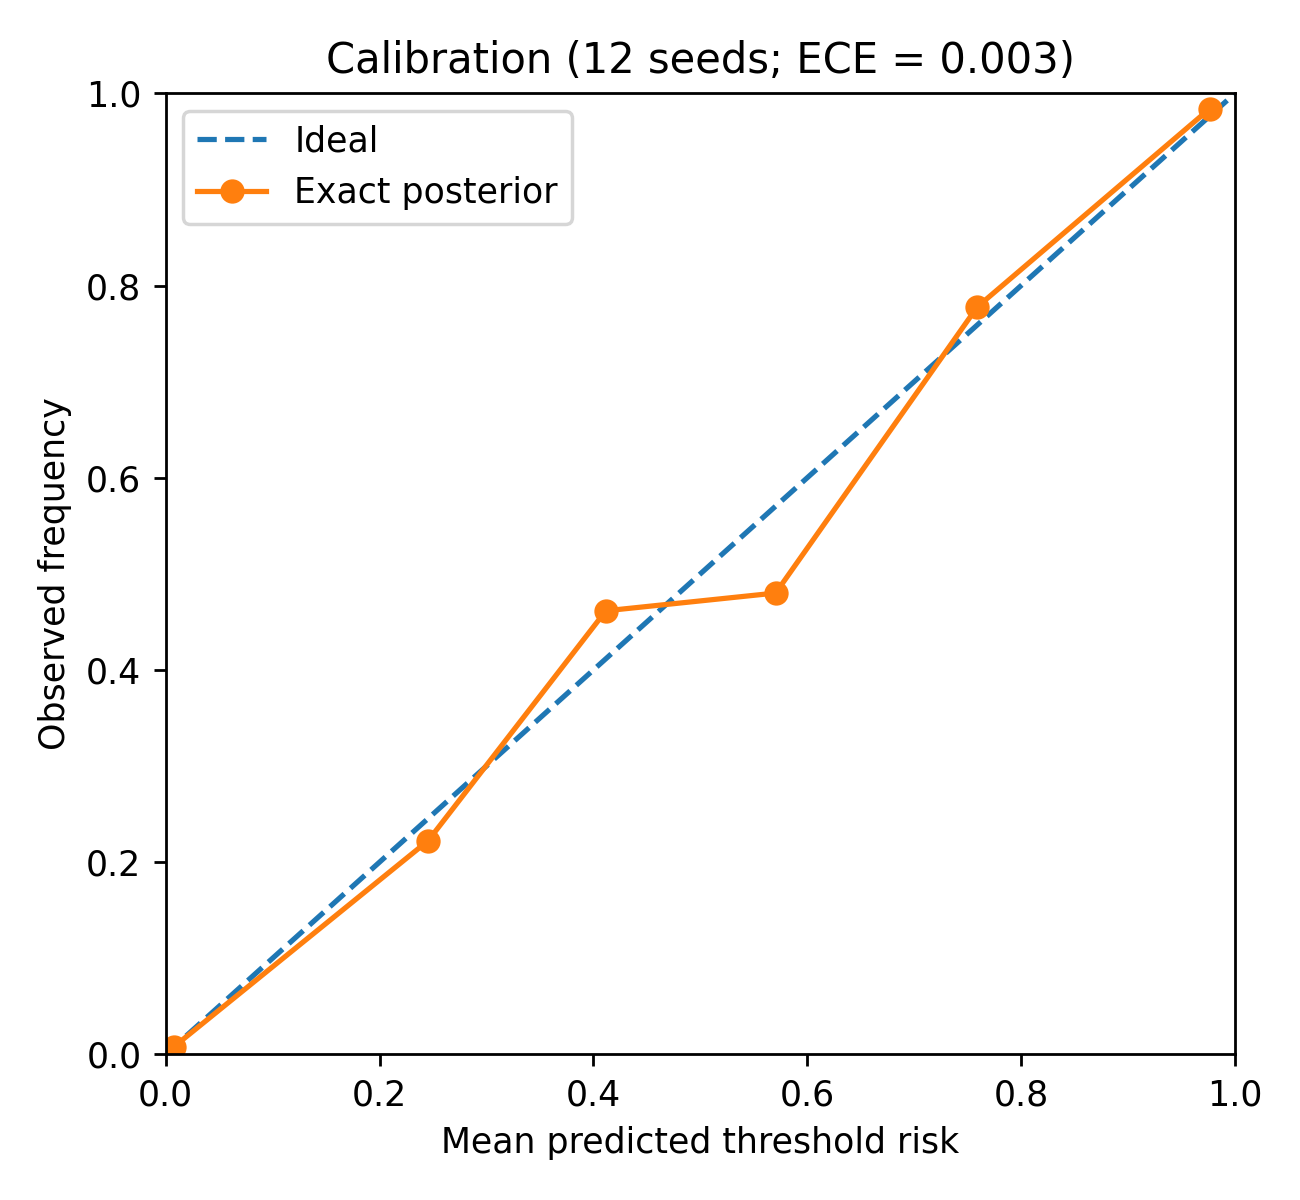
\includegraphics[width=0.86\columnwidth]{figures/calibration.png}
\caption{Posterior calibration under the matched controlled simulator (12 seeds).}
\label{fig:calibration}
\end{figure}

\subsection{Robustness, scale, and action capacity}

\paragraph{Held-out attack-intensity mismatch.} The likelihood contains three declared withholding regimes. We hold out a generator with primary/backup withholding probabilities $(0.65,0.60)$, which is not a likelihood grid point. Across 12 paired seeds, the hierarchical-regime controller reduces the failure-epoch fraction from 0.833 with no reconfiguration to 0.299. A point-likelihood ablation reaches only 0.413. This shows that marginalizing uncertainty in attack intensity is useful when the exact intensity is not known, although it is not evidence of robustness to arbitrary adaptive attacks.

\begin{table}[t]
\caption{Held-out attack-intensity mismatch (12 paired seeds).}
\label{tab:mismatch}
\centering
\small
\begin{tabular}{lcc}
\toprule
Policy & Point likelihood & Regime mixture \\
\midrule
No reconfiguration & 0.833 & 0.833 \\
Random partner & 0.566 & 0.628 \\
\textbf{Risk-aware exchange} & \textbf{0.413} & \textbf{0.299} \\
\bottomrule
\end{tabular}
\end{table}

\paragraph{Scale validation.} We retain the $n=22$ PBFT committee size and run 12 seeds at $K\in\{5,9,18\}$ shards. Because ``any failure'' naturally becomes more likely as $K$ grows, Figure~\ref{fig:scale} reports the true over-threshold shard-epoch fraction. Risk-aware exchange reduces this fraction at every scale: from 0.083 to 0.019 at $K=5$, from 0.148 to 0.051 at $K=9$, and from 0.125 to 0.061 at $K=18$. Decision time grows from 25 ms at $K=5$ to 107 ms at $K=18$ in the simulator, consistent with evaluating a larger finite action set.

\begin{figure}[t]
\centering
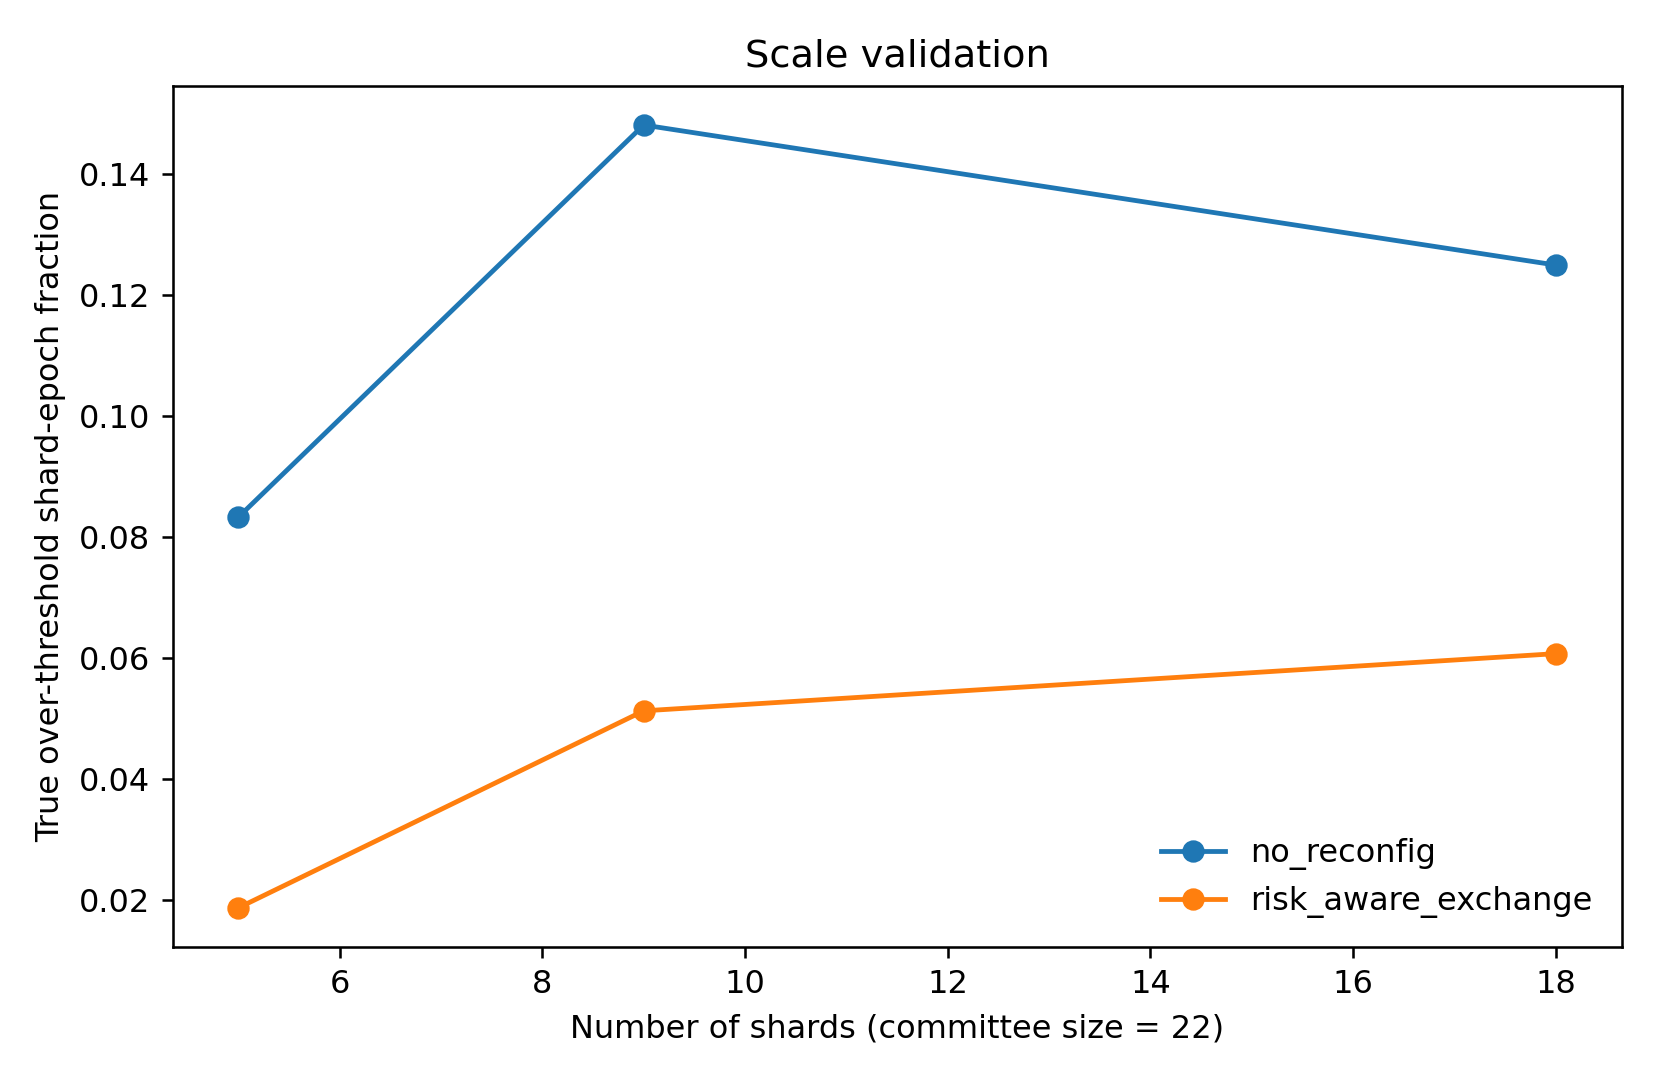
\includegraphics[width=0.92\columnwidth]{figures/scale.png}
\caption{Scale validation with constant 22-validator PBFT committees (12 seeds per scale).}
\label{fig:scale}
\end{figure}

\paragraph{Observation exposure.} We next test whether the progress signal remains useful when each epoch supplies fewer real logical batches.  Under the same held-out attack intensity used above, we vary the observed exposure from 24 to 72 to 216 batches per epoch, without retuning the controller.  Across 12 paired seeds, the risk-aware controller reduces the failure-epoch fraction from 0.833 to 0.490, 0.385, and 0.333, respectively; the paired absolute reductions are 0.344 (95\% CI [0.118, 0.524]), 0.448 ([0.208, 0.656]), and 0.500 ([0.326, 0.660]).  As expected, more observations sharpen the posterior (Brier score falls from 0.052 to 0.020 for the controller), but even the sparse 24-batch setting retains a positive paired effect.  Figure~\ref{fig:exposure} reports the full trend.  This is an evidence-exposure test, not a throughput claim.

\begin{figure}[t]
\centering
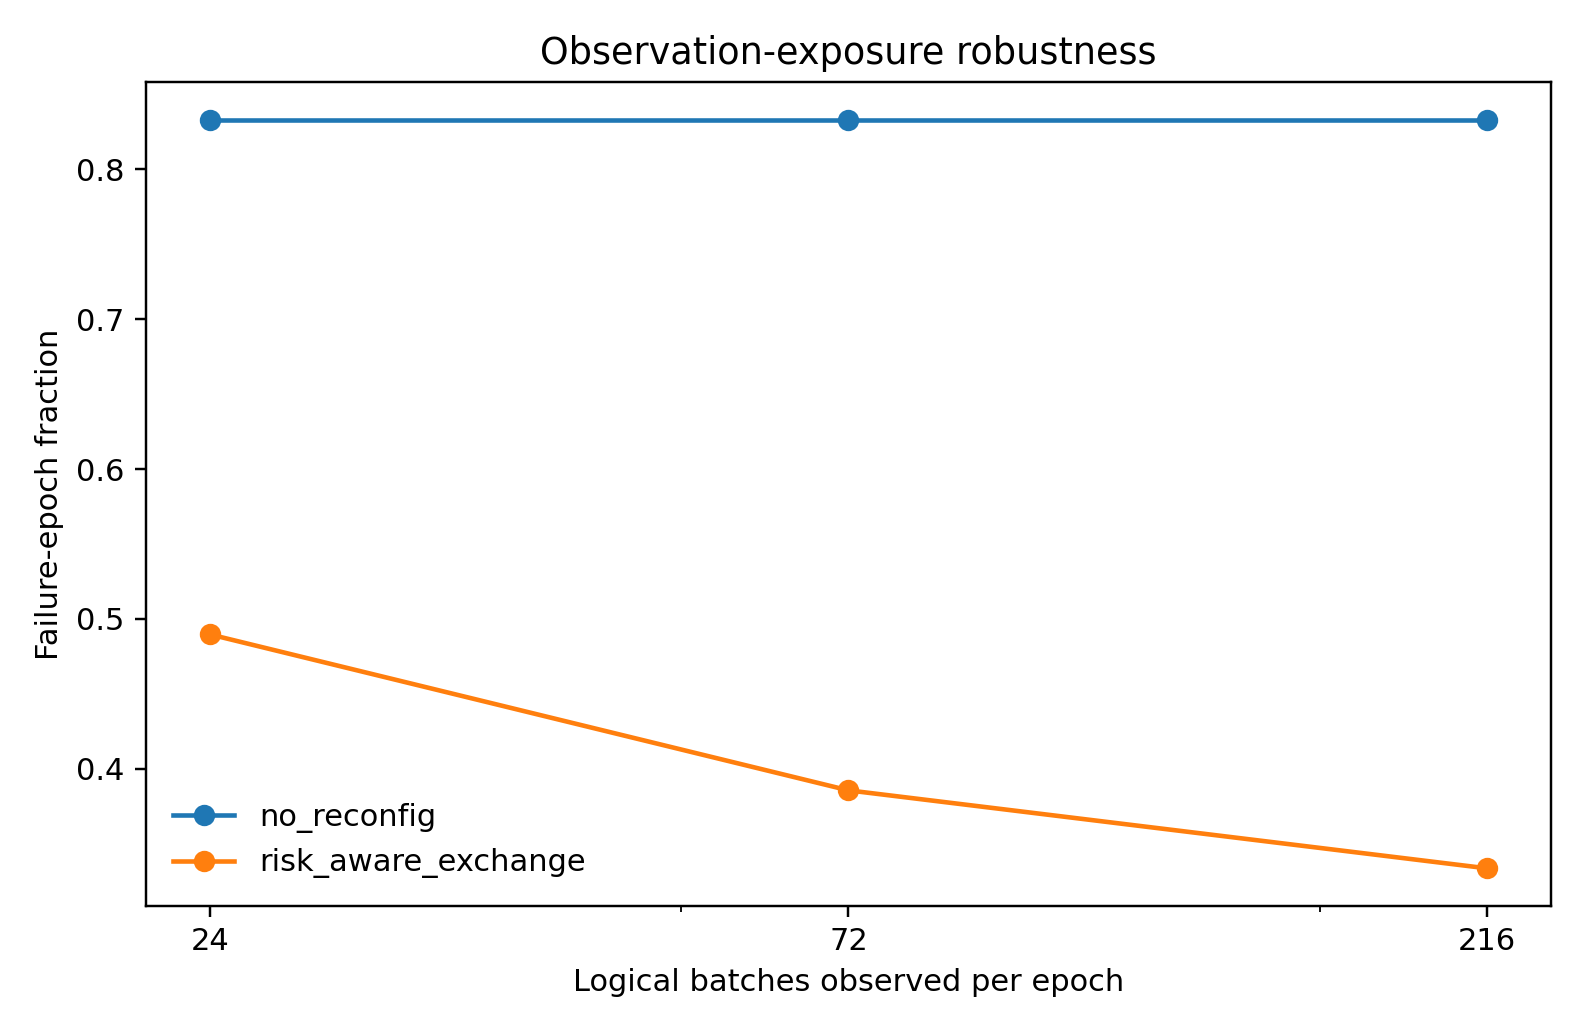
\includegraphics[width=0.92\columnwidth]{figures/exposure.png}
\caption{Observation-exposure robustness under a held-out attack intensity (12 paired seeds).  The controller is unchanged; only the number of logical batches observed per epoch varies.}
\label{fig:exposure}
\end{figure}

\paragraph{Action capacity.} We next vary the true persistent active fraction while retaining $N=198$, $K=9$, and a larger action budget $k\leq6$ to characterize the controller's capacity. Table~\ref{tab:sensitivity} reports 12 paired seeds. The controller reduces failure epochs at active fractions $0.20$, $0.24$, and $0.28$. At $0.32$, both policies fail in every epoch: the local concentration is too severe for the declared exchange budget. This is a useful boundary rather than a hidden negative result. Risk sensing does not create capacity out of nothing; when the system operates too close to the global BFT limit, a small random exchange cannot dilute a high-risk committee fast enough.

\begin{table}[t]
\caption{Persistent-active-fraction sensitivity (12 paired seeds, $k\leq6$).}
\label{tab:sensitivity}
\centering
\scriptsize
\resizebox{\columnwidth}{!}{%
\begin{tabular}{c|cc|c}
\toprule
Active fraction & No reconfig. & \sysname & Moved/epoch \\
\midrule
0.20 & 0.250 & 0.014 & 3.19 \\
0.24 & 0.750 & 0.215 & 5.88 \\
0.28 & 1.000 & 0.549 & 9.13 \\
0.32 & 1.000 & 1.000 & 4.84 \\
\bottomrule
\end{tabular}%
}
\end{table}

\begin{figure}[t]
\centering
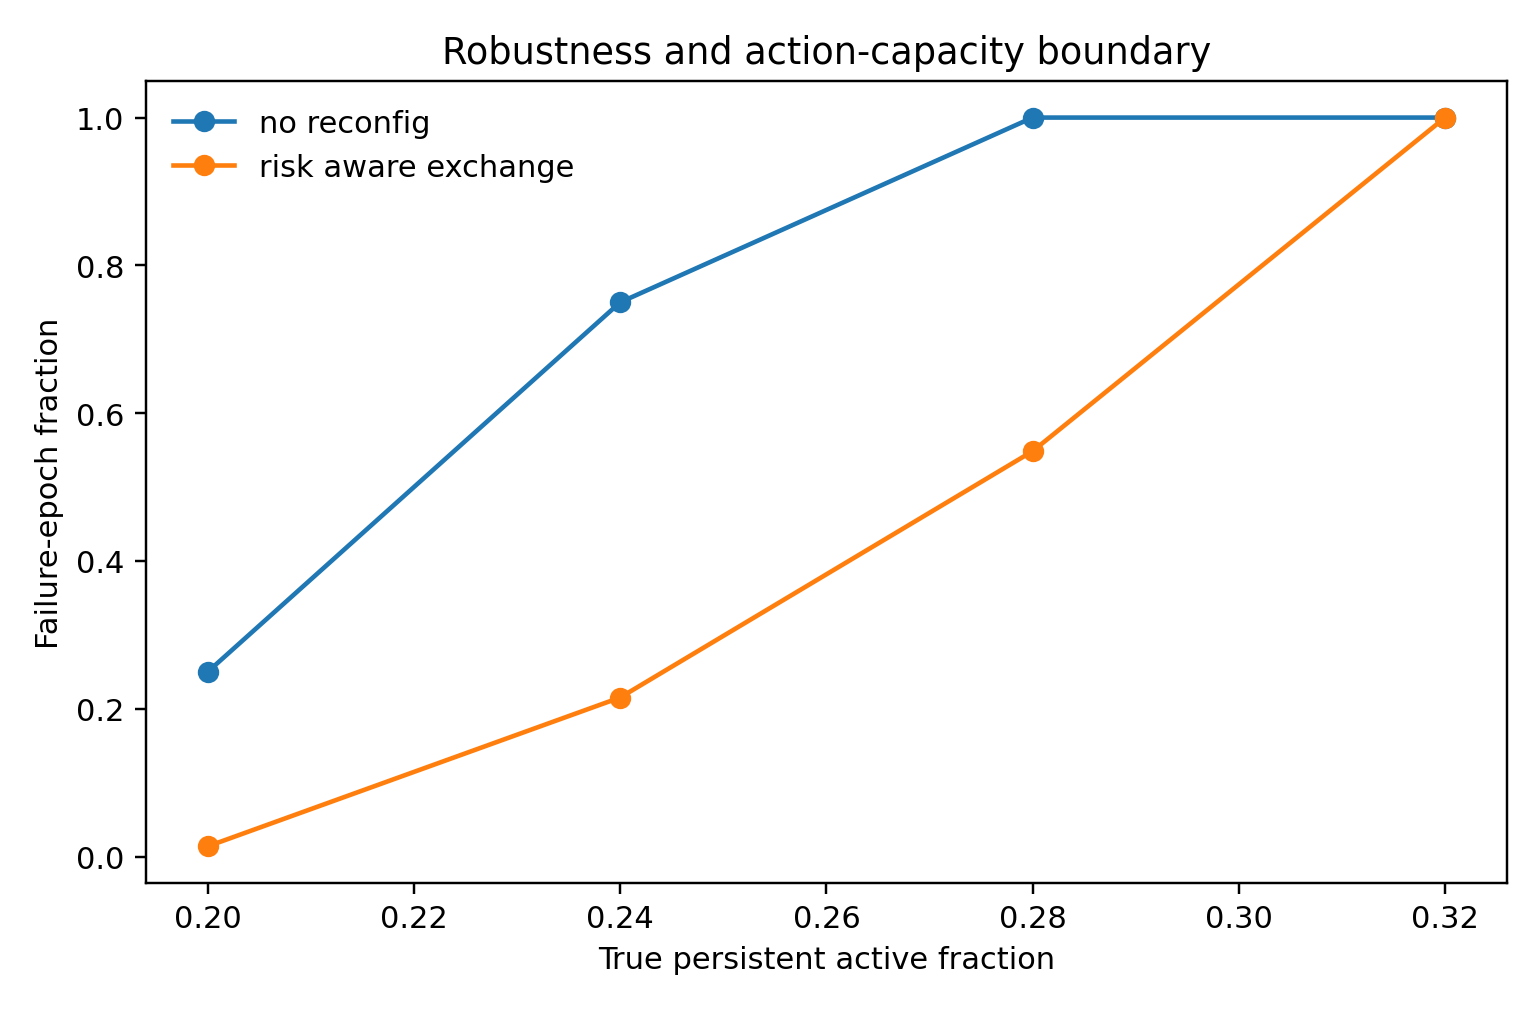
\includegraphics[width=0.92\columnwidth]{figures/sensitivity.png}
\caption{Sensitivity to true persistent active fraction. The failure of the $k\leq6$ controller at 0.32 is an explicit action-capacity boundary.}
\label{fig:sensitivity}
\end{figure}

\paragraph{Threat-budget sensitivity.} The exact posterior requires a configured global active-load budget $L$. The model is valid only when $L$ is an upper bound on the true persistent active load; therefore, we exclude underestimated $L$ from the robustness claim. With true fraction 0.24, conservative configured fractions 0.24, 0.28, and 0.32 yield failure-epoch fractions 0.240, 0.330, and 0.483 across 12 paired seeds. Conservatism is therefore safer in the modeling sense but can reduce control efficiency, motivating a future robust or hierarchical prior over $L$.

\section{Discussion and Limitations}

\paragraph{What the posterior means.} The posterior in \eqref{eq:posterior} is not a claim that runtime logs reveal all Byzantine identities or all latent Byzantine validators. It estimates a persistent, behaviorally active quorum-blocking load under an explicit withholding model. Silent adversaries, adaptive attackers, and unobserved environmental confounders require additional models.

\paragraph{Threat-budget assumption.} Exact inference conditions on a configured global active-load budget $L$. It must be a conservative upper bound rather than an estimate that is allowed to fall below the true persistent active load. The sensitivity result above shows that overly conservative budgets reduce controller efficiency. A production version should maintain a distribution over $L$ or robustly optimize over a range of valid upper bounds.

\paragraph{Reconfiguration cost.} Our controller measures only the logical migration budget and decision time. It does not yet measure membership-view installation, state transfer, checkpoint synchronization, or service interruption. BFT-SMaRt provides an open BFT state-machine replication implementation with reconfiguration support \cite{bftsmart}.  We provide an automated $4\rightarrow5\rightarrow4$ state-transfer and \texttt{currentView}-propagation benchmark harness, but report no handoff number until it has completed on an online BFT-SMaRt runner with its no-op control.

\paragraph{Relationship to corrupted-shard tolerance.} \sysname is complementary to cross-shard tolerance designs. Its purpose is to reduce the frequency or persistence of locally risky shards, not to replace a safety layer that protects the system when a shard is already corrupted.

\section{Conclusion}

This paper introduces a protocol-grounded way to sense PBFT progress without identifying individual validators. By classifying each logical batch as normal, recovered, or stalled, \sysname avoids double-counting the PBFT recovery chain and makes the log-to-risk assumption explicit. An exact constrained Bayesian posterior and a finite random-exchange controller then convert that evidence into a budgeted reconfiguration decision. Controlled simulation suggests that targeted random exchange can reduce local threshold-risk substantially more than blind reshuffling. The remaining path to a submission-quality systems claim is now narrower: execute the provided implementation-level membership-handoff benchmark, broaden network/workload traces beyond the controlled generator, and develop a production treatment of adaptive attackers and uncertain active-load budgets.

\begin{thebibliography}{10}

\bibitem{castro1999pbft}
M. Castro and B. Liskov, ``Practical Byzantine Fault Tolerance,'' in \emph{Proceedings of the Third Symposium on Operating Systems Design and Implementation (OSDI)}, 1999, pp. 173--186.

\bibitem{aublin2013rbft}
P.-L. Aublin, S. Ben Mokhtar, and V. Qu{\'e}ma, ``RBFT: Redundant Byzantine Fault Tolerance,'' in \emph{Proceedings of the 33rd IEEE International Conference on Distributed Computing Systems (ICDCS)}, 2013, pp. 297--306.

\bibitem{omniledger}
E. Kokoris-Kogias, P. Jovanovic, L. Gasser, N. Gailly, E. Syta, and B. Ford, ``OmniLedger: A Secure, Scale-Out, Decentralized Ledger via Sharding,'' in \emph{2018 IEEE Symposium on Security and Privacy}, 2018, pp. 583--598.

\bibitem{rapidchain}
M. Zamani, M. Movahedi, and M. Raykova, ``RapidChain: Scaling Blockchain via Full Sharding,'' in \emph{Proceedings of the 2018 ACM SIGSAC Conference on Computer and Communications Security}, 2018, pp. 931--948.

\bibitem{han2022allocation}
R. Han, J. Yu, and R. Zhang, ``Analysing and Improving Shard Allocation Protocols for Sharded Blockchains,'' in \emph{Proceedings of the 4th ACM Conference on Advances in Financial Technologies}, 2022, pp. 198--216.

\bibitem{cochain}
M. Li, Y. Lin, J. Zhang, and W. Wang, ``CoChain: High Concurrency Blockchain Sharding via Consensus on Consensus,'' in \emph{IEEE INFOCOM 2023 - IEEE Conference on Computer Communications}, 2023, pp. 1--10.

\bibitem{spiralshard}
Y. Lin, M. Li, and J. Zhang, ``SpiralShard: Highly Concurrent and Secure Blockchain Sharding via Linked Cross-shard Endorsement,'' \emph{IEEE/ACM Transactions on Networking}, 2025, doi: 10.1109/TON.2025.3593509.

\bibitem{levee}
X. Wang, Y. Liu, L. Jia, and Y. Sun, ``Levee: A Blockchain Sharding System Capable of Tolerating Faulty Shards,'' \emph{IEEE Transactions on Computers}, vol. 75, no. 2, pp. 477--490, 2026.

\bibitem{bftsmart}
A. Bessani, J. Sousa, and E. Alchieri, ``State Machine Replication for the Masses with BFT-SMART,'' in \emph{2014 44th Annual IEEE/IFIP International Conference on Dependable Systems and Networks}, 2014, pp. 355--362.

\end{thebibliography}
\end{document}
